%
% File acl2015.tex
%
% Contact: car@ir.hit.edu.cn, gdzhou@suda.edu.cn
%%
%% Based on the style files for ACL-2014, which were, in turn,
%% Based on the style files for ACL-2013, which were, in turn,
%% Based on the style files for ACL-2012, which were, in turn,
%% based on the style files for ACL-2011, which were, in turn, 
%% based on the style files for ACL-2010, which were, in turn, 
%% based on the style files for ACL-IJCNLP-2009, which were, in turn,
%% based on the style files for EACL-2009 and IJCNLP-2008...

%% Based on the style files for EACL 2006 by 
%%e.agirre@ehu.es or Sergi.Balari@uab.es
%% and that of ACL 08 by Joakim Nivre and Noah Smith

\documentclass[11pt]{article}
\usepackage{acl2015}
\usepackage{times}
\usepackage{url}
%\usepackage{hyperref}
\usepackage{latexsym}
\usepackage{graphicx}
\usepackage{booktabs}
\usepackage{multirow}

%\setlength\titlebox{5cm}

% You can expand the titlebox if you need extra space
% to show all the authors. Please do not make the titlebox
% smaller than 5cm (the original size); we will check this
% in the camera-ready version and ask you to change it back.


\title{An LSTM Recurrent Network for Step Counting}

\author{Ziyi Chen \\
  Computer Science  \\
  Unversity of California Santa Cruz\\
  {\tt zchen139@ucsc.edu}}
  
  

\date{}

\begin{document}
\onecolumn

%{
%    {\setcounter{page}{0}\renewcommand{\thepage}{\roman{page}}}
%  
%%   % extend down to the page number area (UCSC), which is 1.25in 
%%   % from the bottom
%  \enlargethispage{\footskip}
%
%%    \null\vfil
%  \begin{center}
%  \Large
%    UNIVERSITY OF CALIFORNIA \par
%    \smallskip
%    {\expandafter\uppercase\expandafter{SANTA CRUZ}} \par
%    \bigskip
%    {\bfseries {\expandafter\uppercase\expandafter{An LSTM Recurrent Network for Step Counting}} \par}
%    \medskip
%    A report submitted in partial satisfaction of the \par
%    requirements for the degree of \par
%    \bigskip
%    {\expandafter\expandafter{MASTER OF SCIENCE}} \par
%    \bigskip
%    in \par
%    \bigskip
%    {\expandafter\uppercase\expandafter{COMPUTER SCIENCE}} \par
%    \bigskip
%    by \par
%    \bigskip
%    {\bfseries Ziyi Chen} \par
%    \bigskip
%    December 2017 \par
%  \end{center}
% \setcounter{footnote}{0}

%\vfill
%\begin{center}
%% \fmfont
%\Large
%\hfill \parbox{3in}{The Report of {Ziyi Chen}\\ is approved:} \\
%\bigskip \bigskip \medskip
%\hfill\rule{2.6in}{0.5pt}\\
%\hfill\makebox[2.6in][l]{Professor Roberto Manduchi, Chair }\\
%\bigskip \medskip
%\hfill\rule{2.6in}{0.5pt}\\
%\hfill\makebox[2.6in][l]{Professor Luca de Alfaro, Reader}\\
%\bigskip \smallskip
%\end{center}



\maketitle
\begin{abstract}

Smartphones with sensors such as accelerometer and gyroscope can be used as pedometers and navigators. In this paper, we propose to use an LSTM recurrent network for counting the number of steps taken by both blind and sighted users, based on an annotated smartphone sensor dataset, WeAllWork. The models were trained separately for sighted people, blind people with a long cane or a guide dog for Leave-One-Out training modality. It achieved 5\% overcount and undercount rate.

\end{abstract}

\section{Introduction}

With the increasing ubiquity of smartphones, users are now carrying plenty of sensors with them such as accelerometer, gyroscope, magnetometer, wherever they go. Step counters are being integrated into an increasing number of portable consumer electronic devices such as music players, smartphones, and mobile phones \cite{wiki:pedometer}. There are various of step counting apps on smartphones. Step counters can also be used for estimating the distance and the position in indoor pedestrian navigation systems, which is especially helpful not only for blind people but also for sighted people who need directional information in unfamiliar places.

In this paper, we propose an LSTM model trained with indoor walking sensor data from iPhones, and annotated data generated by shoe-mounted sensors (MetaWear-CPRO) from the WeAllWalk dataset, to predict the number of steps. The MetaWear-CPRO units are attached to the uesr's shoes so they can provide precise heel strike times. In the dataset, blind volunteers using a long cane or a guide dog and sighted volunteers have different gait patterns, so we built the models separately for each group of walkers and measured the performances based on three error metrics. We also tested the accuracy of those models by using leave-one-out cross-validation. Three error metrics splitting intervals differently were used for measuring the overcount and undercount rates of the system. We tried different parameters for the LSTM models such as the number of training steps and window size to find the best settings. The model achieved 1\% overcount and undercount rate on a mixed dataset and 5\% under the Stratified Leave-One-Out training modality.



\section{Background and Related Work}

\subsection{Step Counting}

\begin{figure*}[htb]
\centering
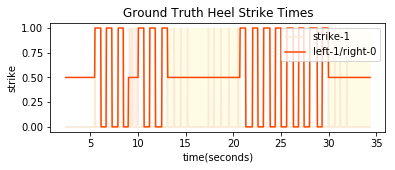
\includegraphics[scale=0.5]{ground_truth_2}
\caption{An example of heel strike times in T1\_ID1\_WC.xml from 2.4s to 34.4s. The first step at 5.4761s is a left step. A feature motion (the participant walked into the wall, stopped, and moved to the left) happened during 9.041862s to 10.041862s. Then one turn from east to south and another turn from south to east occurred during 13.1752s to 20.7419, and 30.0419s to 39.1419s respectively. Feature data, turn data, and all data recorded before the first step are removed.}
\label{fig:ground_truth}
\end{figure*}


Automatic step counting has received substantial attention in both research and commercial domains. There is a wealth of studies on the use of inertial sensors for detecting and characterizing walk-related activities. Pedometers are usually portable and electronic or electromechanical \cite{wiki:pedometer}. They can be embedded in shoes, in smartwatches, in smartphones, and attached to users' ankles or hung on the belt.

\cite{brajdic2013walk} evaluated common walk detection (WD) and step counting (SC) algorithms applied to smartphone sensor data. The results favor the use of standard deviation thresholding (WD) and windowed peak detection (SC) with error rates of less than 3\%.
\cite{tomlein2012advanced} introduced step detection and intelligent detection of cheating based on smartphone sensors.
\cite{naqvib2012step} presented a method for counting the number of steps taken by a user using the smartphone-based accelerometer while walking at any variable speed.

With the rapid development of deep learning, this advanced technology is used in various fields including step counting. Since sensors provide time series data, researchers have tried to use RNN for counting the number of steps. \cite{edel2015advanced} uses Bidirectional Long Short-Term Memory Recurrent Neural Networks (BLSTM-RNNs) for step detection, step length approximation as well as heading estimation.

In addition to sighted people, some researchers also pay attention to people with visual impairment. \cite{haegele2015validation} validated Centrios talking pedometer for adolescents with different level of visual impairment under the daily-living condition, while  \cite{holbrook2011validation} validated the same talking pedometer for adults.



\subsection{The WeAllWalk Dataset}

The WeAllWalk dataset \cite{flores2016weallwalk} contains sensor data gathered from ten blind participants with a long cane or a guide dog and five sighted participants. The smartphone (iPhone 6s) carried by participants recorded the sensor data. Two small sensors attached to the participants’ shoes recorded heel strike times as the labels. Each segment of paths is marked as either a straight segment or a turn segment. Special circumstances on the road are also labeled as features. \cite{flores2016weallwalk} have tested six different algorithms for step counting and turn detection. 


\section{Implementation}
We propose an LSTM model trained with indoor walking sensor data from iPhone for step counting. Since blind participants using a long cane or a guide dog and sighted volunteers have different gait patterns, we build the models separately and calculate the error rates by using three metrics. Also, we only consider straight segments in the paths, since the gait pattern is more likely to be regular than the gait pattern of turn segments, and remove segments marked as features such as opening a closed door and avoiding an obstacle. We try different parameters for the LSTM model and add a dropout layer to make the result more robust.

\subsection{Data Preprocessing}

\begin{figure*}[ht]
\centering
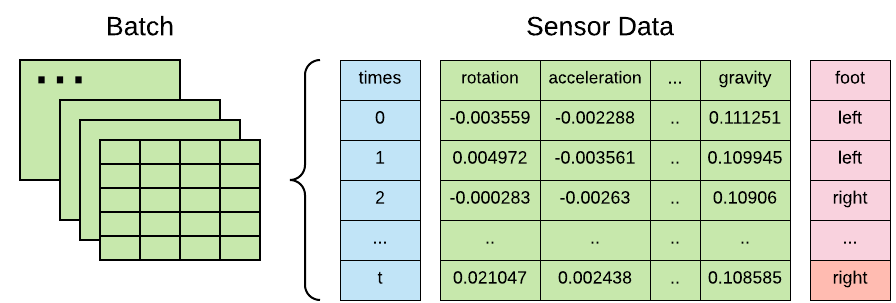
\includegraphics[scale=1]{input2}
\caption{Input (green) and output (pink) samples for our model. The model uses the latest t records of the sensor data (green blocks) to predict the current status (the last pink block). The first t-1 predictions of each segment are from the intermediate outputs (light pink) of the recurrent neural network, since they do not have t records for prediction as the rest do.}
\label{fig:batch_sensor_data}
\end{figure*}

We use two kinds of files from the dataset. The first type is CSV format iPhone sensor data.  Each CSV file contains the sensor data recorded with a path and a person. There are 39 columns of sensor data and some of them are more useful than others. So we select 6 columns (rotationRateX, rotationRateY, rotationRateZ,  userAccelerationX, userAccelerationY, userAccelerationZ) from the sensor data to building our model. 

The second type is XML file containing annotated ground truth data for paths walked by each participant. Each file contains tags of start time, end time and direction for each segment the participant walked through. For each segment, the time and foot of each step are recorded, and special situation such as moving to the wall is also marked as feature with start time, end time and detailed description. We only train and test the step counting system with the segments recorded when participants traverse straight in each path, where gait patterns are assumed to be regular. We also remove time slots that have been marked as feature. 

Since the XML files only contain heel strike times and it's very difficult to predict heel strike times with the sensor data, we can not use them as the labels directly. If we regard the labels at heel strike times as 1s and the labels at other points in time as 0s, then the labels are too unbalanced to train a model to predict the labels at each point in time. So we transform the XML files to binary signals in which left steps toggle the signal from 0 to 1 and right steps toggle the signal from 1 to 0 as shown in Figure \ref{fig:ground_truth}.

Finally, we windowed the data (window size is equal to the number of timesteps) for corresponding sensor data and ground truth signals to generate the formatted training data and labels.


\subsection{The LSTM Model}
Long short-term memory (LSTM) network is a time-recursive neural network, suitable for processing and predicting important properties of time series data. LSTM has many applications in the science and technology domains. LSTM-based systems can learn tasks such as translating natural languages, image analysis, speech recognition, controlling chat robots and so on.

LSTM network is a special kind of recurrent neural network (RNN). The main difference between LSTM and RNN lies in that LSTM adds a "processor" to judge whether the information is useful or not in the algorithm. The structure of this processor is called cell.

Three non-linear units (an input gate, a forget gate and an output gate) are placed in the cell. When a message enters the LSTM network, the system would determine whether the message is useful or not. Only information that complies with algorithmic requirements will remain, and misleading information will be forgotten through the forget gate.


\begin{figure}[ht]
\centering
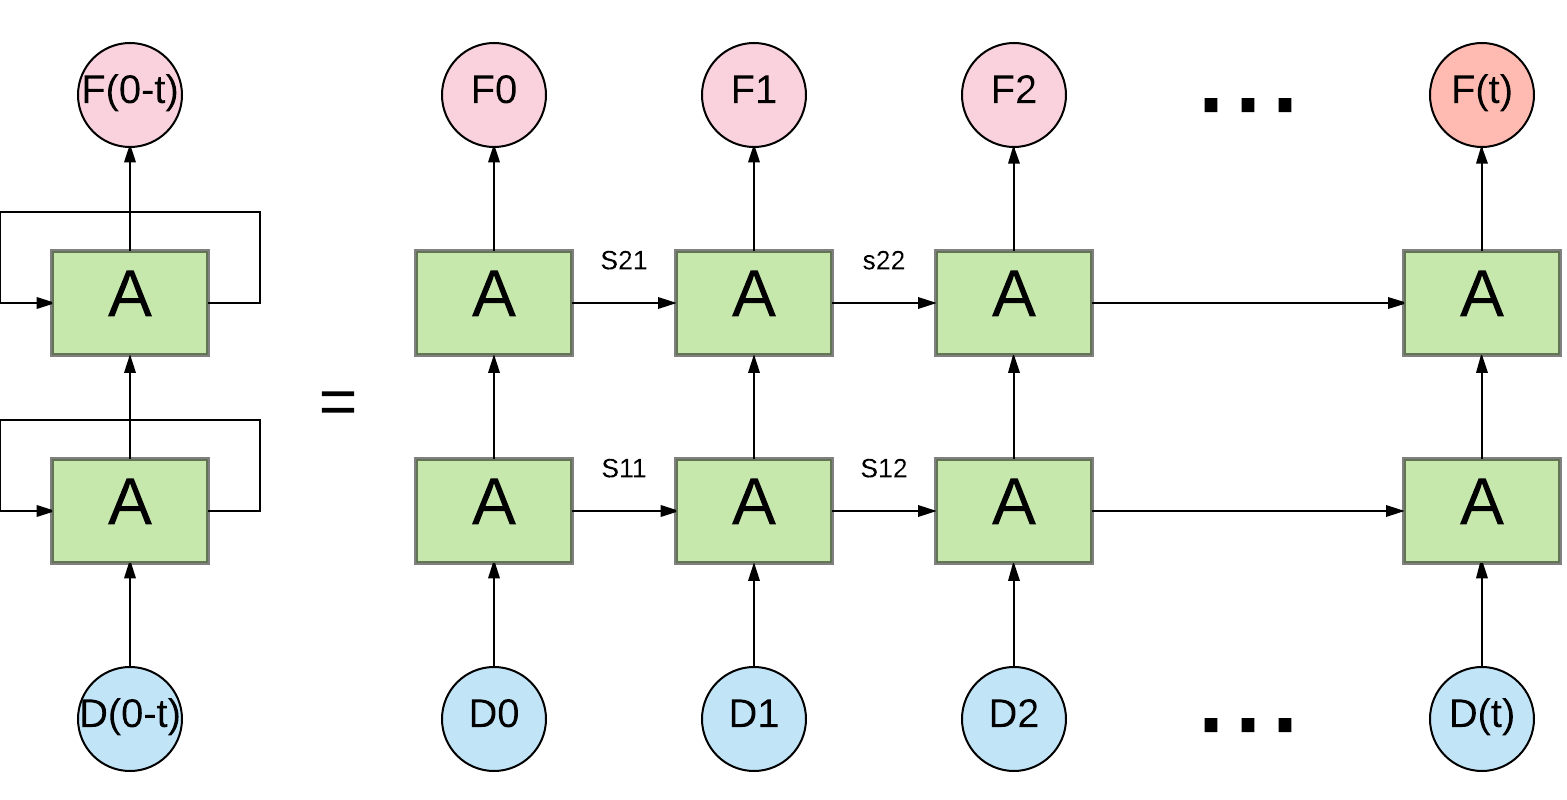
\includegraphics[scale=0.3]{LSTM3}
\caption{A two-layer LSTM recurrent network. Each green block is an LSTM cell. Blue circle D(t) represents the sensor data recorded at time t while s is the inner LSTM state, and pink circle F is the output. Each LSTM cell receives the input of current sensor data and state from previous cell (the initial state is 0), and outputs a state and an output.}
\label{fig:LSTM}
\end{figure}

\begin{figure*}[ht]
\centering
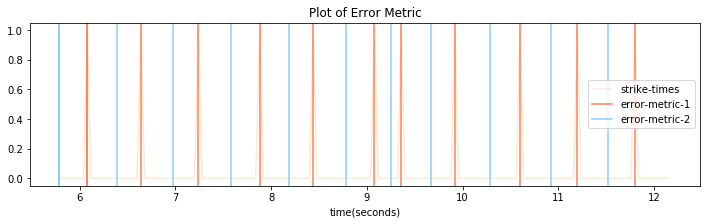
\includegraphics[scale=0.6]{error_metric}
\caption{An example of three error metrics. Assume above plot is an entire segment. Error metric 1 (red line) divides segments into intervals exactly at each heel strike time. Error metric 2 (blue line) divides intervals at the center point of every pair of adjacent heel strike times. Both error metric 1 and 2 compute undercount and overcount rates for each interval independently while error metric 3 calculates undercount and overcount rates within the entire segment.}
\label{fig:error_metric}
\end{figure*}

We use TensorFlow to implement the LSTM network. TensorFlow is an open-source software library that can be used for machine learning applications such as neural networks \cite{wiki:tensorflow}. It supports both CPU and GPU and it provides an interface in Python. TensorFlow uses a data flow graph to represent computation in terms of the dependencies between individual operations \cite{tensorflow.org}. We first define the data flow graph and then create a session to run the graph. The saver class can save and restore the values of graph variable to and from checkpoints by mapping variable names to tensor values.

As shown in Figure \ref{fig:LSTM}, a two-layer RNN network with 2 basic LSTM cells is built for training with mean squared error loss function. 
As shown in Figure \ref{fig:batch_sensor_data}, the input batch is a list of matrices. Each row of the matrices is a list of sensor data at a point in time. The length of the list is called the number of timesteps.
For example, if we want to use the sensor data recorded at the latest 50 points in time to predict the current label, each sensor data contains input size ($6$ in our model) values of rotation rate and user acceleration in 3-dimension. So the matrix size is the number of timesteps multiply input size which is $50 \times 6$. All such matrices form the input list and are transformed to tensor as the training data. Since the dataset is big and there are more than one hundred thousand elements in the input list which would make the training process very slow, we shuffle and divide training data into small batches (batch size = 256) and feed the batches to the optimizer one step by one step.

There are two ways to get the outputs. The first one is to use the latest 50 inputs to predict the current output. The second way is to use the intermediate outputs of RNN to generate predictions. The first one can not predict the first 50-1 labels, but it is more precise since more information is used to produce one output. We use the first way to predict all other labels.


\begin{figure*}[ht]
\centering
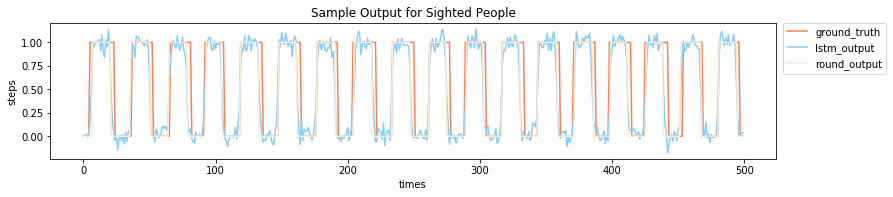
\includegraphics[scale=0.5]{output_sighted}
\caption{Sample output from mixed data for all sighted people. The origin output signal (blue line) swings near 0 or 1. The round signal (yellow line) is quite similar to the ground truth data (red line).}
\label{fig:output_sighted}
\end{figure*}



\subsection{Error Metrics}

The original result signal is a list of float numbers around 0 to 1. Then we transform the signal into a binary signal where the value is either 0 or 1. And the predicted heel strike times is the signal change times. Now we can calculate the accuracy rate of the result, which is the proportion of correct predictions (1 is predicted as 1 or 0 is predicted as 0) in total predictions. The error rate of the step counting model was measured using three different metrics as shown in Figure \ref{fig:error_metric}. The error metric 1 and 3 are as same as the error metrics proposed in \cite{flores2016weallwalk}.

The first metric splits intervals at each real heel strike times and counts the number of predicted steps within each time interval $[T_i, T_{i+1}]$.  If exact one step is detected within each interval, the count of the step is correct. If no step is detected during the interval, then one undercount event happens. If $n$ steps are detected during the interval, then $n-1$ overcount events are recorded. The undercount and overcount rate is the number of undercount events or overcount events divided by the total number of real steps.

The second metric is similar to the first one,  but it  splits intervals at the center point of two adjacent ground-truth heel strike times, and counts the number of predicted steps within each time interval $[\frac{T_{i-1}+T_i}{2}, \frac{T_i+T_{i+1}}{2}]$. The undercount and overcount rate is calculated in a same way as the first metric does. As shown in Figure \ref{fig:output_small_metric2} at the end of this paper,  the metric can decrease error rate when one step is detected sightly earlier ($t_i<T_i$) and the next step is detected sighted later ($t_{i+1}<T_{i+1}$). In this case, interval $[T_i, T_{i+1}]$ has one undercount event, and interval $[T_{i-1}, T_i]$ and $[T_{i+1}, T_{i+2}]$ have one overcount event.

The third metric counts the number of predicted steps during each segment and compares to the number of ground-truth steps during the same segment. If the ground-truth number is larger, then undercount events happen. If the predicted number is larger, then overcount events happen. The undercount and overcount rate is calculated by dividing the sum of undercount events and overcount events by the number of all steps in ground truth. The undercount and overcount rate obtained by the error metric 3 is always smaller than or equal to the corresponding values computed by the metric 1 and 2.

\begin{figure*}[ht]
\centering
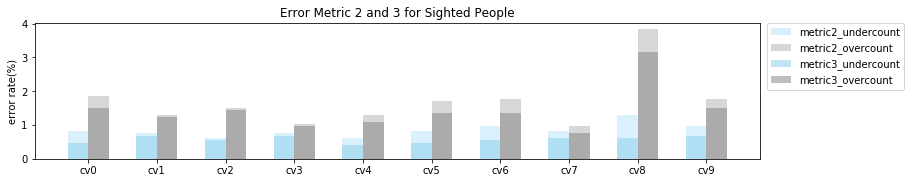
\includegraphics[scale=0.5]{error_metric_23_na_10fold}
\caption{Error rates measured in error metric 2 and 3 under 10-fold cross-validation on mixed data for all sighted people. The error rate of metric 2 is always higher than metric 3. The undercount error rate (blue blocks) is less than overcount error rate(grey blocks). Detailed values are shown in table \ref{label_metric23_sighted}.}
\label{fig:error_metric_23_na_10fold}
\end{figure*}

\begin{figure*}[ht]
\centering
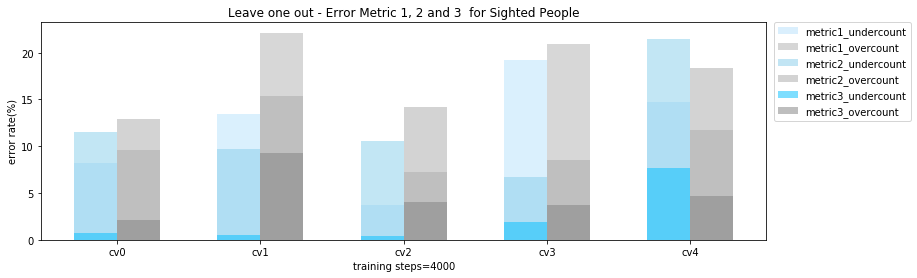
\includegraphics[scale=0.5]{error_metric_123_na_5fold}
\caption{Error rates measured in error metric 1, 2 and 3 for leave-one-out data of sighted people.}
\label{fig:error_metric_123_na_5fold}
\end{figure*}


\section{Experiments}

We preprocessed the WeAllWalk data to train the LSTM model for the different communities by using two ways of splitting training and testing data. The first way is to simply mix all data and split it into the training set and testing set. In this way, both the training and the testing data contain records from all participant and all segments. The second way is leaving one person out, which means testing set contains and only contains all records from one participant while the training set contains all other records from the remaining participants.

The model is trained with different sensor data, numbers of timesteps, output size, numbers of hidden layers, optimizers, learning rates and numbers of training steps. We first try different optimizers with various learning rates and find that AdamOptimizer with a learning rate around 0.01 can make the loss converged, and then fix the optimizer. 


\subsection{Sighted people}
There are more than 120,000 valid records from sighted walkers, we split it into 100,000 records of training data and 25,000 records of testing data. Each input is a 3-dimensional tensor, with a shape of batch size $\times$ number of timesteps $\times$ number of sensor signals.

For mixed data, we apply 10-fold cross-validation. A good result sample is shown in Figure \ref{fig:output_sighted}. The output signal swings near 0 or 1. So it is reasonable to round the signal ($>0.5$ turn to 1, $<=0.5$ turn to 0). The rounded signal is similar to the ground truth data. However, not all results are as good as in this sample. Some of the bad results are shown at the end of the paper. Some results have a certain offset between the real heel strike time and the predicted heel strike time, some result curves shake more fiercely so that not all values are close to 0 or 1. There tend to be more strikes if the output value shakes around 0.5. So in our experiments, the overcount rate is always higher than the overcount rate.

\begin{figure}[ht]
\centering
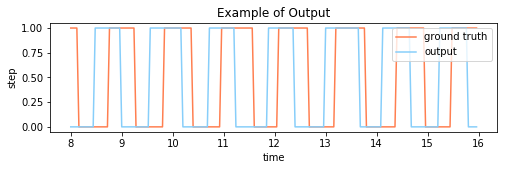
\includegraphics[scale=0.4]{output_ex_offset}
\caption{Sample output of offset. In this case, error metric 1 works better than error metric 2.}
\label{fig:output_ex_offset}
\end{figure}


Since there are 6 error rates, it is difficult to determine an overall measurement combining all error rates and tell which model is better. All 10 results are shown in Figure \ref{fig:error_metric_23_na_10fold}.
The average undercount rate measured in metric 3 is around 0.6\%, and the average overcount rate measured in metric 3 is around 1.4\%.  
The average undercount rate measured in metric 2 is around 0.9\%, and the average overcount rate measured in metric 2 is around 1.7\%.  
The value of error rate is shown in table \ref{label_metric23_sighted}. The error rate measured in metric 1 is much higher than error rate measured in metric 2 and 3, the undercount rate measured in metric 1 is similar to overcount rate measured in metric 1 (around 20\%) as shown in Figure \ref{fig:error_metric_1_na_10fold}. The reason that caused such situation is described in Figure \ref{fig:output_small_metric2}. In metric 1, undercount and overcount error rates are similar since a undercount event is usually followed by a overcount event and vice versa.

\begin{figure}[ht]
\centering
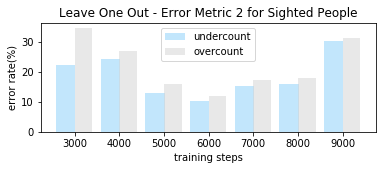
\includegraphics[scale=0.55]{error_metric_2_na_step}
\caption{Error rates measured in metric 1 and 3 under 10-fold cross-validation with sighted people data. The error rate measured in metric 1 is always higher than in metric 3.}
\label{fig:error_metric_2_na_step}
\end{figure}


\begin{figure*}[ht]
\centering
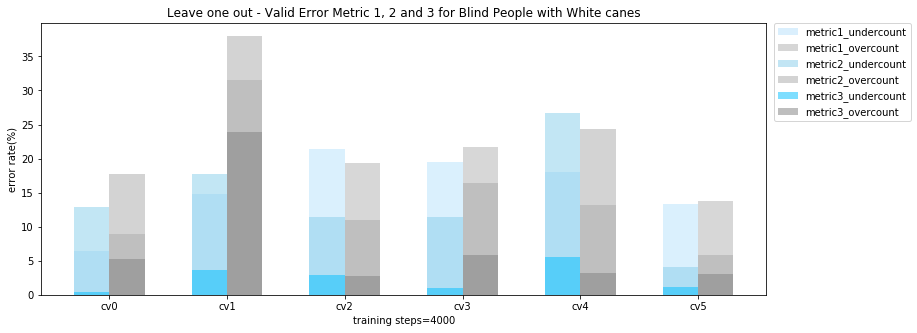
\includegraphics[scale=0.5]{error_metric_wc_10fold_valid4000}
\caption{Error rates on blind people with a long cane leave-one-out validation set.}
\label{fig:error_metric_wc_10fold_valid4000}
\end{figure*}


\begin{figure*}[ht]
\centering
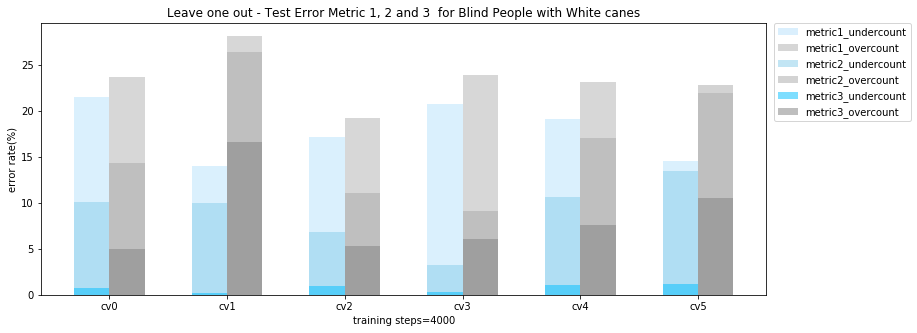
\includegraphics[scale=0.5]{error_metric_wc_10fold_test4000}
\caption{Error rates on blind people with a long cane leave-one-out testing set.}
\label{fig:error_metric_wc_10fold_test4000}
\end{figure*}

For leave one person out method, the cross-validation result is shown in Figure \ref{fig:error_metric_123_na_5fold}.
The average undercount rate in metric 3 is around 2.5\%. The average overcount rate in metric 3 is around 7\%.
In some cases, metric 2 has bad performances, because there is an offset around half of each interval as shown in the Figure \ref{fig:error_metric_2_na_step}. 
In the experiments with different parameters of LSTM model, on some validation sets (cv3 performs best in most of the experiments) the model achieves overcount and undercount rates less than 0.1\% in metric 3, while less than 1\% in metric 1 or 2. But for other validation sets, the overcount rate is extremely high (30\% to 60\%). Each validation set has a better performance with models with different parameters. It might because different people have different gait patterns. So I choose the model where each validation set has an average performance. 

When both the training and testing data contain the sensor data from all people, the predicted signal is quite accurate, and the error rate (in metric 2 and 3) of step counting is small. However, with the leave-one-out method, there would be offsets for both training and testing data, and the accuracy of predicted signal is low. But the error rate in metric 1 could be small if the offset is similar for each heel strikes as shown in Figure \ref{fig:output_ex_offset}. 

\subsection{Blind People with a long cane}
There are more than 120,000 records from blind people with a long cane, participants 1, 2, 3, 5, 6, 7, 8 have sensor data for six paths. So we use data from participant 8 as the testing data, and records from all remaining people as the training and validation data for 6-fold leave-one-out cross-validation. The validation and testing results are shown in Figure \ref{fig:error_metric_wc_10fold_valid4000} and \ref{fig:error_metric_wc_10fold_test4000}. All error rates are higher than on the mixed data. The good performance from the validation data does not mean that the model can have a good performance on the testing data.
The training dataset only contains data from 6 different people, which is not a big number. If we have annotated data from more people, the LSTM model might detect more walking patterns of blind people and provide a better result.

\begin{figure*}[ht]
\centering
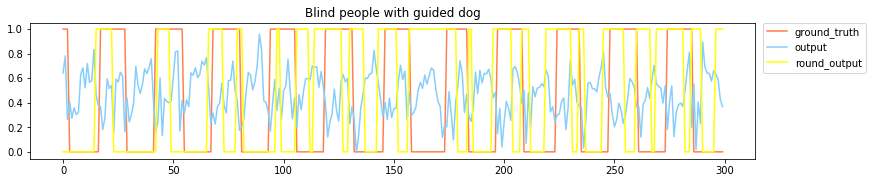
\includegraphics[scale=0.5]{blind_gd}
\caption{Sample output on blind people with guide dog.}
\label{fig:blind_gd}
\end{figure*}


\subsection{Blind people using a guide dog}

There are only 3 people walking with a guide dog. Each of them generates 30,000 records of sensor data. So we regard the data from two people as the training data and those from the left one as the testing data. The result is bad as shown in \ref{fig:blind_gd}. Although the model shows a  good performance on mixed data (error rate is around 5\% in metric 2 and 2\% in metric 3), it is difficult to predict the strike heel times of a person with a model trained with the data from only one other person.

\begin{table}[]
\centering
\caption{Error rates on blind people with a guide dog}
\label{my-label}
\begin{tabular}{llll}
\hline
error(\%)                &            & valid & test  \\ \hline
metric1                  & undercount & 23.90 & 10.18 \\
                         & overcount  & 26.14 & 25.75 \\ \hline
\multirow{2}{*}{metric2} & undercount & 22.56 & 12.27 \\
                         & overcount  & 29.03 & 19.49 \\ \hline
\multirow{2}{*}{metric3} & undercount & 4.52  & 0.53  \\
                         & overcount  & 10.98 & 17.75 \\ \hline
\end{tabular}
\end{table}


\section{Conclusion and Future Work}

We trained an LSTM model using annotated smartphone sensor data from the WeAllWalk dataset to count steps. In the dataset, blind volunteers using a long cane or a guide dog, sighted volunteers have different gait patterns, so we separately built the models and calculated the error rates in three metrics. We also applied leave-one-out pedometers to test the accuracy of our models by using three error metrics, that split intervals differently to compute the number of overcounted and undercounted steps. The model achieved 1\% overcount and undercount rate on the mixed training data and 5\% under leave-one-out training modality.

As shown in Figure \ref{fig:overcount} and Figure \ref{fig:undercount}, simply rounding the origin output signal might cause overcount or undercount event. So we can use a better way to transform the signal into a binary signal. In this paper, we only use the data of straight segments by removing turn segments and other features. We could consider turn segments and feature motions in the future. We now only use rotation rate and user acceleration as the input, we can also try more features in the dataset in the future.

\begin{figure}[ht]
\centering
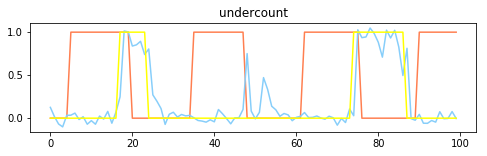
\includegraphics[scale=0.4]{undercount}
\caption{Sample of undercounting.}
\label{fig:undercount}
\end{figure}

\begin{figure}[ht]
\centering
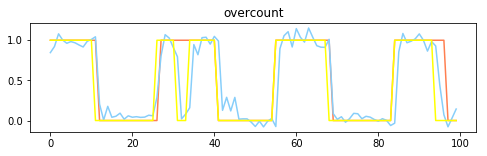
\includegraphics[scale=0.4]{overcount}
\caption{Sample of overcounting.}
\label{fig:overcount}
\end{figure}


\begin{figure*}[ht]
\centering
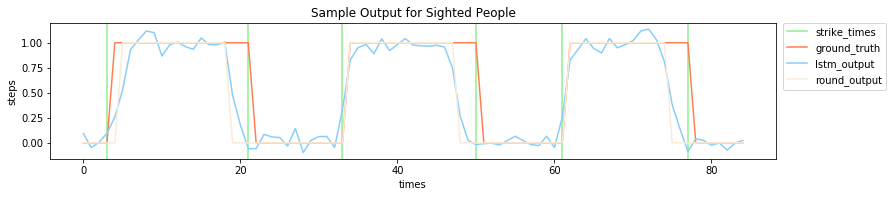
\includegraphics[scale=0.5]{output_small_metric2}
\caption{A bad sample in error metric 1. The green line splits the intervals in error metric 1. There are random offsets between actual strike times and predicted strike times. In this case, the first, third and fifth interval has one overcount while the second and the fourth intervals have one undercount.}
\label{fig:output_small_metric2}
\end{figure*}




\begin{figure*}[ht]
\centering
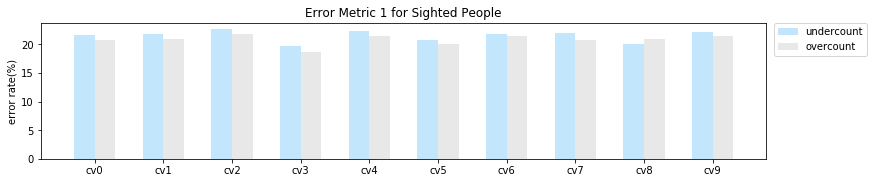
\includegraphics[scale=0.5]{error_metric_1_na_10fold}
\caption{Error metric 1 under 10-fold cross-validation on sighted people. The error rate is much higher than the error rate in metric 2 and 3 as shown in this figure. The reason that caused such situation is also described in tge figure.}
\label{fig:error_metric_1_na_10fold}
\end{figure*}


\begin{figure*}[ht]
\centering
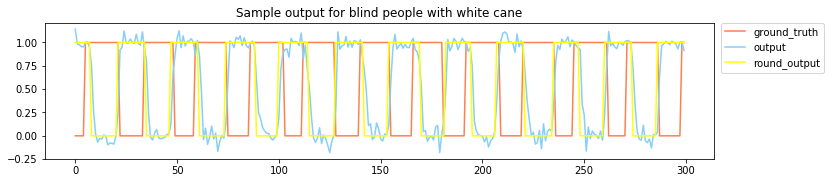
\includegraphics[scale=0.5]{output_wc_1}
\caption{An output sample on blind people with a long cane.}
\label{fig:output_wc_1}
\end{figure*}

\begin{figure*}[ht]
\centering
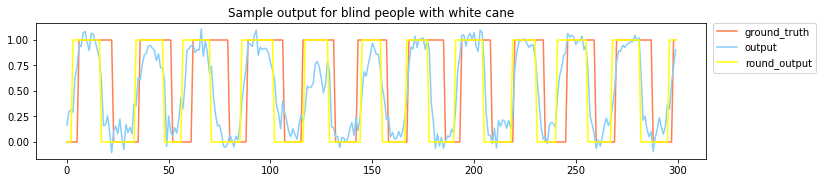
\includegraphics[scale=0.5]{output_wc_2}
\caption{An output sample on blind people with a long cane.}
\label{fig:output_wc_2}
\end{figure*}




\begin{table*}[]
\centering
\caption{Performance measured in metric 2 and 3 under 10-fold cross-validation on sighted people}
\label{label_metric23_sighted}
\begin{tabular}{llllllllllll}
\hline
error(\%)                &            & cv0   & cv1   & cv2   & cv3   & cv4   & cv5   & cv6   & cv7   & cv8   & cv9  \\ \hline
metric1                  & undercount & 0.82  & 0.75  & 0.62  & 0.75  & 0.62  & 0.82  & 0.96  & 0.82  & 1.3   & 0.96 \\
                         & overcount  & 1.85  & 1.3   & 1.5   & 1.03  & 1.3   & 1.71  & 1.78  & 0.96  & 3.83  & 1.78 \\ \hline
\multirow{2}{*}{metric2} & undercount & 0.48  & 0.68  & 0.55  & 0.68  & 0.41  & 0.48  & 0.55  & 0.62  & 0.62  & 0.68 \\
                         & overcount  & 1.5   & 1.23  & 1.44  & 0.96  & 1.09  & 1.37  & 1.37  & 0.75  & 3.15  & 1.5  \\ \hline
\end{tabular}
\end{table*}


\begin{table*}[]
\centering
\caption{Performance measured in mertric 1, 2 and 3 on blind people using a long cane}
\label{my-label}
\hspace*{-1.5cm}
\begin{tabular}{|l|l|l|l|l|l|l|l|l|l|l|l|l|l|}
\hline
\multicolumn{2}{|l|}{\multirow{2}{*}{error(\%)}} & \multicolumn{2}{l|}{cv0} & \multicolumn{2}{l|}{cv1} & \multicolumn{2}{l|}{cv2} & \multicolumn{2}{l|}{cv3} & \multicolumn{2}{l|}{cv4} & \multicolumn{2}{l|}{cv5} \\ \cline{3-14} 
\multicolumn{2}{|l|}{}                           & valid       & test       & valid       & test       & valid       & test       & valid       & test       & valid       & test       & valid       & test       \\ \hline
\multirow{2}{*}{m1}       & undercount      & 6.44        & 21.49      & 14.83       & 14.03      & 21.45       & 17.1       & 19.5        & 20.67      & 18.05       & 19.03      & 13.35       & 14.56      \\ \cline{2-14} 
                               & overcount       & 8.87        & 23.63      & 31.5        & 28.1       & 19.32       & 19.2       & 21.69       & 23.91      & 13.17       & 23.09      & 13.7        & 21.94      \\ \hline
\multirow{2}{*}{m2}       & undercount      & 12.93       & 10.09      & 17.79       & 9.97       & 11.36       & 6.77       & 11.49       & 3.28       & 26.69       & 10.62      & 4.09        & 13.45      \\ \cline{2-14} 
                               & overcount       & 17.81       & 14.36      & 38.01       & 26.33      & 10.97       & 11.07      & 16.37       & 9.06       & 24.35       & 17.06      & 5.9         & 22.76      \\ \hline
\multirow{2}{*}{m3}       & undercount      & 0.43        & 0.7        & 3.63        & 0.21       & 2.94        & 0.94       & 1.03        & 0.29       & 5.59        & 1.11       & 1.2         & 1.19       \\ \cline{2-14} 
                               & overcount       & 5.32        & 4.96       & 23.85       & 16.57      & 2.7         & 5.25       & 5.9         & 6.07       & 3.25        & 7.55       & 3.01        & 10.5       \\ \hline
\end{tabular}
\end{table*}


\nocite{*}


% include your own bib file like this:
\bibliographystyle{acl_natbib}
\bibliography{acl2015}





\end{document}





















